\newif\ifusingieee
\IfFileExists{IEEEtran.cls}{\usingieeetrue\documentclass[conference]{IEEEtran}}{\usingieeefalse\documentclass[10pt,twocolumn]{article}}
\ifusingieee\else\usepackage[margin=0.70in,columnsep=0.25in]{geometry}\fi
\providecommand{\IEEEauthorblockN}[1]{#1\\}
\providecommand{\IEEEauthorblockA}[1]{\small #1}
\makeatletter
\@ifundefined{IEEEkeywords}{\newenvironment{IEEEkeywords}{\par\small\noindent\textbf{Keywords: }}{\par}}{}
\makeatother
\usepackage{booktabs}
\usepackage{graphicx}
\usepackage{amsmath}
\usepackage{hyperref}
\usepackage{xcolor}
\usepackage{array}
\usepackage{multirow}

\title{GNN-BERT Fusion for Musical Context Understanding from Audio Structure and Text Metadata}

\author{\IEEEauthorblockN{Maskat Ibne Wahid, Zannaty Aziza, Abdur Rahman Piash}
\IEEEauthorblockA{Department of Computer Science and Engineering\\
BRAC University, Dhaka, Bangladesh\\{}
Group 7, Section 4; IDs: 22299224, 24241316, 22201583}}

\begin{document}
\maketitle

\begin{abstract}
Music context depends on both acoustic structure and semantics. This work studies a supervised hybrid architecture that combines a GraphSAGE representation of music segments with contextual text representations from DistilBERT. Each track is divided into five-second segments. A segment becomes a graph node described by log-mel, chroma, MFCC, energy, and spectral statistics; temporal adjacency and acoustic similarity define edges. Text contains leakage-safe track, album, and artist metadata. We compare a random predictor, a mel-spectrogram CNN, BERT-only, GNN-only, early concatenation, and graph-to-text cross-attention on 1,000 tracks selected from the official FMA-small split. Performance is measured with Macro-F1, Micro-F1, and area under the precision-recall curve. The repository also produces threshold-tuned evaluation, t-SNE embeddings, graph samples, and three qualitative attention case studies. The CNN was strongest on the 100-track test subset, reaching 0.382 Macro-F1 and 0.477 Macro AUC-PR; early concatenation was the best fusion variant at 0.331 Macro-F1. These results show that the implemented fusion is functional but that sparse metadata did not improve on direct acoustic modeling in this limited run.
\end{abstract}

\begin{IEEEkeywords}
music information retrieval, graph neural network, BERT, multimodal fusion, GraphSAGE
\end{IEEEkeywords}

\section{Introduction}
Musical identity is not encoded in one representation. A spectrogram exposes timbre and frequency energy, sequential features show local temporal change, metadata expresses semantic clues, and repeated sections establish long-range relationships. Conventional convolutional systems are effective at local time-frequency patterns, but their grid structure does not directly express that a chorus near the end resembles one near the beginning. A graph can represent such non-local relationships explicitly, while a language model can encode the contextual meaning of text associated with a track.

This project investigates whether these views are complementary. Our audio branch treats fixed-length segments as graph nodes and uses GraphSAGE message passing. The text branch uses DistilBERT to encode a short sentence assembled from track title, album title, and artist name. We test two fusion choices: early concatenation of pooled branch representations and cross-attention in which the graph embedding queries contextual token embeddings.

The main contributions are: (1) a reproducible segment-graph pipeline using temporal and similarity edges; (2) a leakage-safe paired audio-text construction from FMA; (3) a controlled six-model comparison on identical data splits; and (4) qualitative analysis connecting graph structure, token attention, and predicted labels. Unlike a generative music system, the objective is supervised context understanding.

\begin{figure*}[t]
\centering
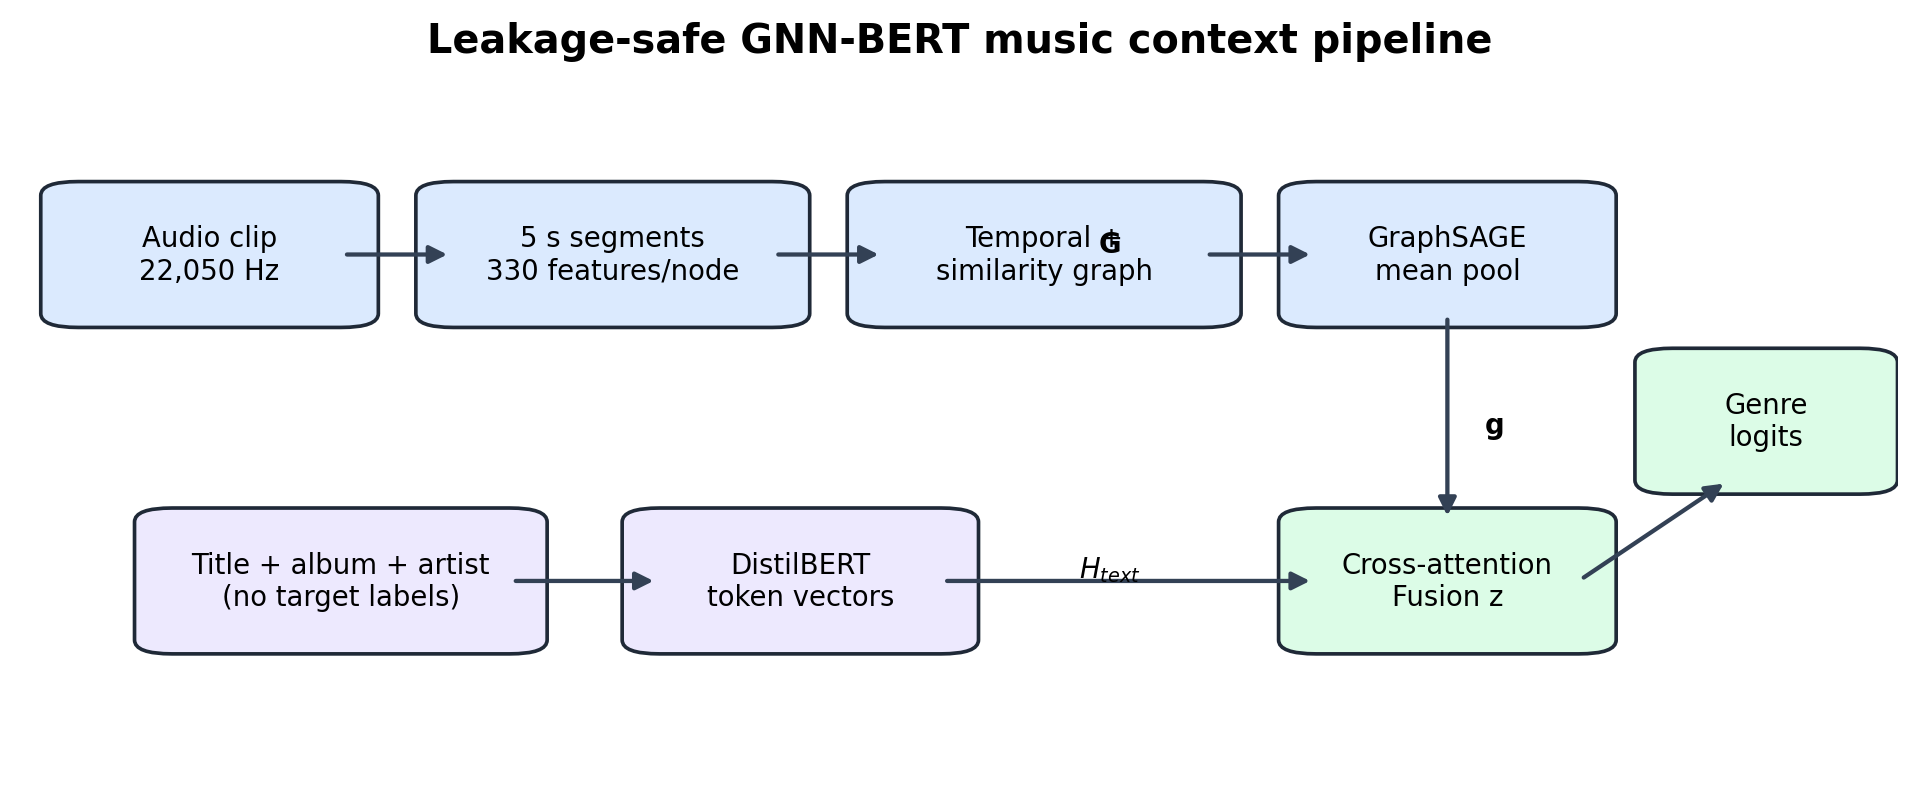
\includegraphics[width=0.92\textwidth]{../plots/architecture_pipeline.png}
\caption{End-to-end pipeline. The audio branch creates a segment graph and pooled structural representation $g$. The text branch produces contextual token embeddings $H_{text}$ without exposing target genre words. Cross-attention combines both representations before classification.}
\label{fig:pipeline}
\end{figure*}

\section{Related Work}
The Free Music Archive (FMA) dataset introduced a large, open benchmark containing audio, hierarchical genres, and extensive metadata \cite{defferrard2017fma}. Its predefined subsets and splits make it suitable for reproducible genre experiments. The small subset is balanced across eight top-level genres and is computationally feasible on a hosted GPU notebook.

BERT learns bidirectional contextual language representations through transformer pretraining \cite{devlin2019bert}. DistilBERT preserves much of BERT's language capability in a smaller model produced by knowledge distillation \cite{sanh2019distilbert}. We use it because the assignment requires a BERT-family encoder while Colab memory and runtime are limited.

GraphSAGE is an inductive GNN that learns to aggregate neighborhood information rather than assigning an independent embedding to every graph node \cite{hamilton2017graphsage}. This is appropriate because every track produces a previously unseen segment graph. PyTorch Geometric supplies the message-passing and batch pooling implementation \cite{fey2019pyg}. Audio features are computed with librosa \cite{mcfee2015librosa}.

\section{Dataset and Leakage Control}
\subsection{FMA-small}
The experiment uses FMA-small audio clips and the paired official metadata tables. The deadline-feasible run processed 1,000 tracks: 800 training, 100 validation, and 100 test examples. No track failed decoding. Decode failures are logged and removed before model training, ensuring every model sees the same valid examples.

The default target is an eight-dimensional one-vs-rest vector corresponding to FMA's balanced top-level genres. Although exactly one label is positive for each FMA-small track, representing targets as a binary vector keeps the same loss and evaluation interface required for multi-label context prediction. The implementation can additionally learn a training-only vocabulary from the hierarchical \texttt{genres\_all} field for a genuinely multi-label extension.

\subsection{Text construction}
The text sentence contains only track title, album title, and artist name. Genre columns, genre IDs, and any target-derived descriptions are excluded. This prevents trivial leakage in which BERT reads the answer. Empty fields are skipped and fully empty rows receive a neutral ``Unknown music track'' string.

We retain FMA's official training, validation, and test designation. Track-ID intersections are asserted to be empty. Artist intersections are reported rather than hidden because the official split, required by the project brief, may not be fully artist-disjoint. All threshold selection and early stopping use validation data; the test split is evaluated once per selected checkpoint.

\section{Audio Graph Construction}
Audio is resampled to 22,050 Hz, converted to mono, peak-normalized, padded or truncated to 29 seconds, and divided into five-second segments. For every segment we compute 128-bin log-mel energy, 12-bin chroma, 20 MFCC coefficients, spectral centroid, bandwidth, rolloff, RMS energy, and zero-crossing rate. Mean and standard deviation over time are concatenated, producing 330 features per node. Features are standardized within each track.

Let $x_i$ denote node $i$. Bidirectional temporal edges connect $i$ and $i+1$. To capture repeated sections, non-adjacent pairs are compared using cosine similarity. An edge is added when similarity exceeds $0.80$, with at most two strongest similarity neighbors per node. Similarity becomes the stored edge weight, while temporal edges have weight one. The GraphSAGE layers use connectivity; saved weights support analysis and future weighted variants.

For layer $l$, the update is
\begin{equation}
h_i^{(l+1)}=\sigma\left(W^{(l)}[h_i^{(l)}\Vert \operatorname{mean}_{j\in\mathcal{N}(i)}h_j^{(l)}]\right).
\end{equation}
Three layers with batch normalization, ReLU, and dropout are followed by global mean pooling to obtain track vector $g$.

\section{Models}
\subsection{Baselines}
The random/prevalence baseline samples scores influenced by label frequencies learned only from training data. The CNN receives normalized log-mel spectrograms and contains four convolution, batch-normalization, ReLU, and max-pooling blocks followed by adaptive pooling. BERT-only classifies the DistilBERT first-token representation. GNN-only classifies $g$. These baselines separate local acoustics, text semantics, and graph structure.

\subsection{Early concatenation}
The early-fusion model concatenates the pooled graph vector and DistilBERT first-token vector:
\begin{equation}
z=\operatorname{LayerNorm}(\operatorname{Dropout}(\operatorname{ReLU}(W[g\Vert t]+b))).
\end{equation}
A linear head returns one logit per genre.

\subsection{Cross-attention fusion}
The primary model projects $g$ to one query and projects every contextual token vector to keys and values. Four-head attention calculates
\begin{equation}
A=\operatorname{softmax}\left(\frac{QK^\top}{\sqrt{d}}+M\right), \qquad c=AV,
\end{equation}
where $M$ masks padded tokens. The classifier receives $[g\Vert c]$. Unlike early concatenation, this permits the audio representation to select which text tokens contribute to the fused context.

\subsection{Training objective}
All supervised networks minimize class-weighted binary cross-entropy with logits:
\begin{equation}
\mathcal{L}=-\frac{1}{K}\sum_{k=1}^{K}w_k[y_k\log\sigma(s_k)+(1-y_k)\log(1-\sigma(s_k))].
\end{equation}
Weights use the negative-to-positive frequency ratio in training data and are capped at 20. AdamW, gradient clipping, mixed precision, and early stopping are used. The lower DistilBERT layers are frozen; trainable transformer parameters receive a smaller learning rate than new GNN and classifier parameters. Every pseudorandom generator is seeded.

\begin{table}[t]
\caption{Hyperparameters used in the reported run.}
\centering
\begin{tabular}{lr}
\toprule
Setting & Value \\
\midrule
Audio sample rate & 22,050 Hz \\
Segment duration & 5 s \\
Mel bins / MFCCs & 128 / 20 \\
Similarity threshold / top-$k$ & 0.80 / 2 \\
GraphSAGE layers / width & 3 / 192 \\
Fusion width / attention heads & 192 / 4 \\
Dropout & 0.30 \\
New-layer learning rate & $10^{-3}$ \\
BERT learning rate & $2\times 10^{-5}$ \\
Maximum epochs / patience & 5 / 5 \\
\bottomrule
\end{tabular}
\label{tab:hyperparameters}
\end{table}

\section{Implementation and Reproducibility}
The repository separates acquisition, preprocessing, datasets, architectures, training, evaluation, visualization, and inference. Configuration is centralized in a YAML file. Each processed manifest row stores track ID, official split, artist ID, raw audio path, leakage-safe text, label vector, graph path, mel path, and node count. Graph objects are serialized as PyTorch Geometric \texttt{Data} values, while at least 20 compact JSON versions are exported for inspection and submission.

Preprocessing is resumable: existing graph and mel tensors are reused unless feature settings change. Every decode exception is recorded with track ID rather than silently ignored. A separate audit asserts unique track IDs and zero track overlap among the three official partitions. This audit also reports artist overlap. Model checkpoints include weights, model type, input dimension, number of labels, threshold, and a copy of the effective configuration, so inference does not depend on undocumented defaults.

The training runner applies the same early-stopping rule to every learned baseline. The random baseline uses a fixed seed and training prevalence only. Label weights are calculated from training targets. Threshold selection reads validation predictions only. Test probabilities and embeddings are saved in compressed arrays, enabling metric recalculation without retraining. The included unit tests verify audio feature dimensions and finite values, bidirectional temporal edges, CNN/GNN tensor shapes, cross-attention shape, and metric bounds.

Two execution profiles reduce avoidable computational cost. The reported profile processed 1,000 tracks for five epochs on a Tesla T4. A larger profile is configured for all valid FMA-small tracks and up to 20 epochs, but it was not used because of the submission-time constraint. The split audit found no duplicate track IDs and no track or artist overlap among the selected official partitions. All five learned models completed five epochs; their trainable parameter counts ranged from 277,448 for GraphSAGE to 14,860,424 for cross-attention.

\section{Evaluation Protocol}
Macro-F1 averages label-level F1 scores and therefore exposes weak minority-label performance. Micro-F1 pools all binary decisions. Macro AUC-PR averages label-wise average precision and is informative under class imbalance. A single decision threshold is selected from $0.10$ to $0.90$ using validation Macro-F1, then fixed for test evaluation. We also report exact label-set match as a strict supplementary measure.

The required ablation compares BERT-only, GNN-only, early concatenation, and cross-attention. CNN supplies the no-graph/no-text audio baseline, while the random method provides a lower bound. All methods share processed examples and splits. Training curves are stored for auditability. t-SNE \cite{vandermaaten2008tsne} visualizes the final fused embedding but is used as qualitative evidence rather than a quantitative metric.

For each trainable model, Fig.~\ref{fig:curves} plots training and validation binary cross-entropy together with validation Macro/Micro-F1. We interpret both final test performance and validation behavior for signs of underfitting or overfitting. Parameter counts and wall-clock duration are secondary costs, because a small metric change may not justify a much larger multimodal model.

\section{Results}
\begin{table}[t]
\caption{Test-set comparison for the reported 1,000-track run.}
\centering
\scriptsize
\setlength{\tabcolsep}{3pt}
\IfFileExists{generated_results_table.tex}{\input{generated_results_table.tex}}{\begin{tabular}{lc}\toprule Status & Value \\ \midrule Final run & Required \\ \bottomrule\end{tabular}}
\label{tab:results}
\end{table}

\begin{figure}[t]
\centering
\IfFileExists{../plots/model_comparison.png}{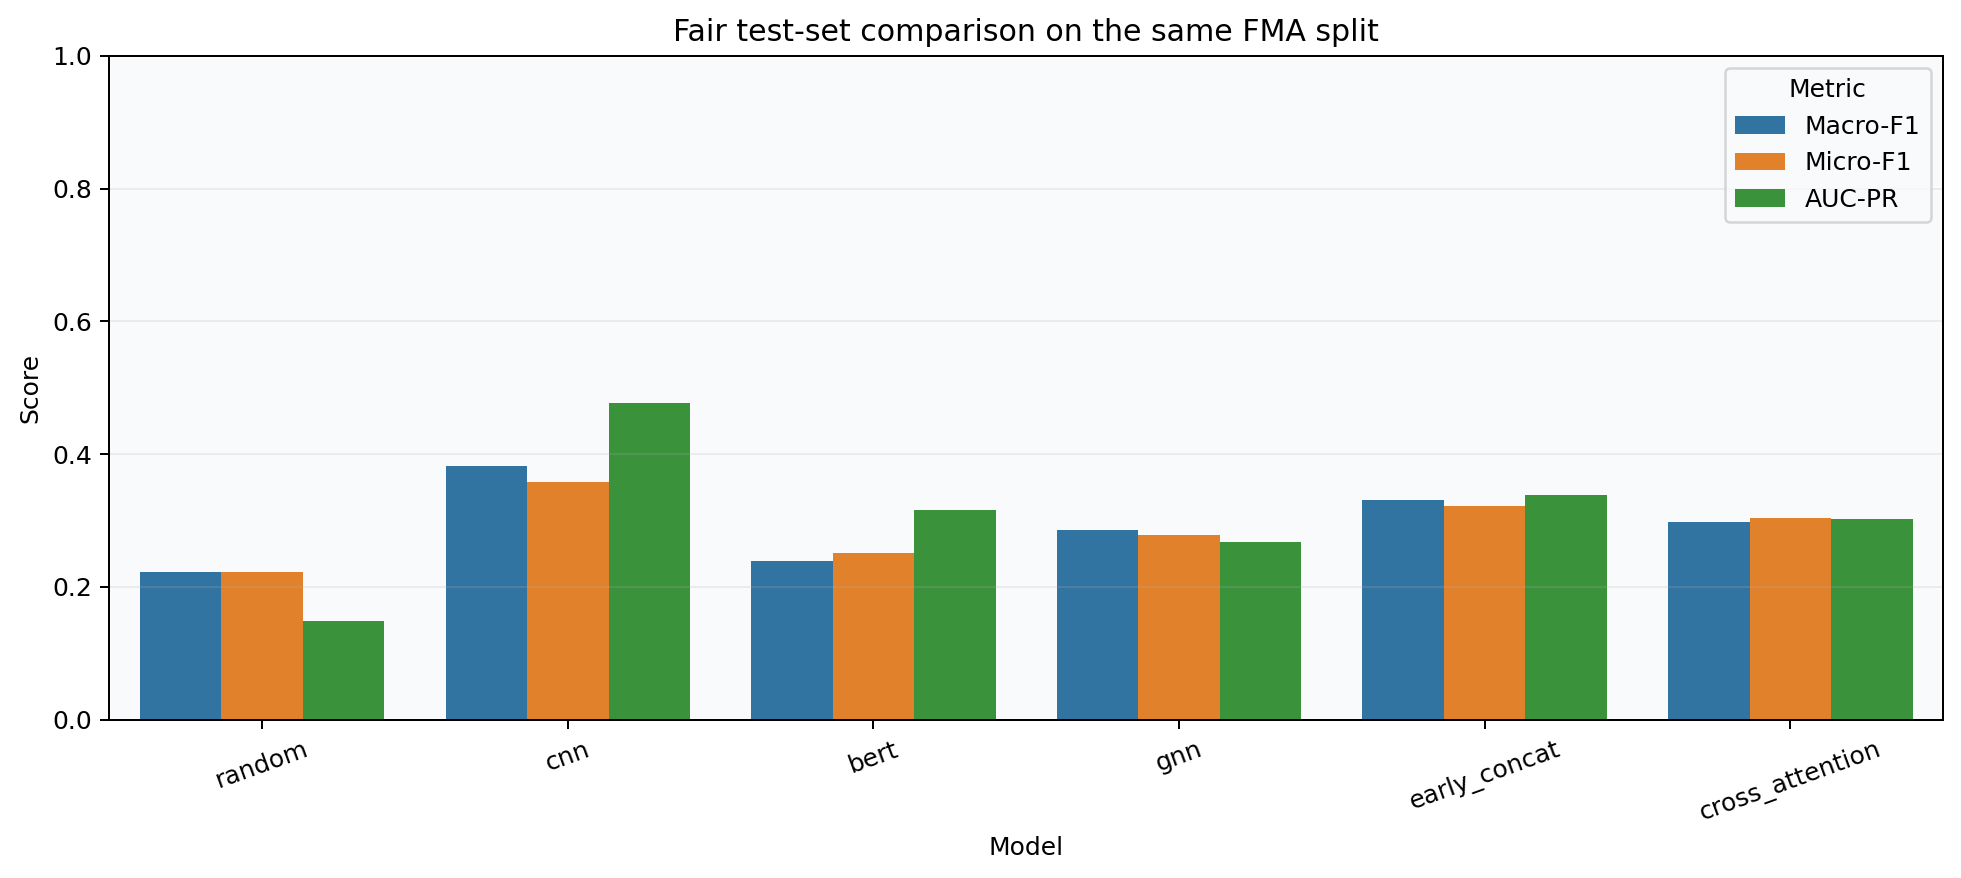
\includegraphics[width=\columnwidth]{../plots/model_comparison.png}}{\fbox{\parbox[c][1.8in][c]{0.9\columnwidth}{\centering Comparison plot unavailable.}}}
\caption{Macro-F1, Micro-F1, and Macro AUC-PR under a shared test split.}
\label{fig:comparison}
\end{figure}

The CNN produced the best result: 0.382 Macro-F1, 0.358 Micro-F1, and 0.477 Macro AUC-PR. GraphSAGE improved Macro-F1 over the random predictor by 0.064 (0.286 versus 0.222), showing that the segment graph learned useful structure, but it remained 0.096 below the CNN. BERT-only obtained 0.239 Macro-F1 and 0.315 AUC-PR, indicating that leakage-safe title, album, and artist text was informative but insufficient by itself.

Early concatenation was the strongest multimodal model at 0.331 Macro-F1, 0.321 Micro-F1, and 0.338 AUC-PR. It exceeded both BERT-only and GNN-only in Macro-F1, yet remained 0.051 below the CNN. Cross-attention reached 0.298 Macro-F1 and therefore did not consistently improve fusion; it was 0.033 below early concatenation. Its greater flexibility appears to overfit the small training subset: validation Macro-F1 peaked at epoch 3 (0.428), while later validation loss increased. The same pattern appears for BERT and early concatenation. Training time was modest on the T4 (13--25 seconds per learned model after preprocessing), but the BERT-based models used about 14--15 million trainable parameters compared with 0.28--0.32 million for the GNN and CNN. Therefore their lower test scores do not justify the additional complexity in this run.

\begin{figure*}[t]
\centering
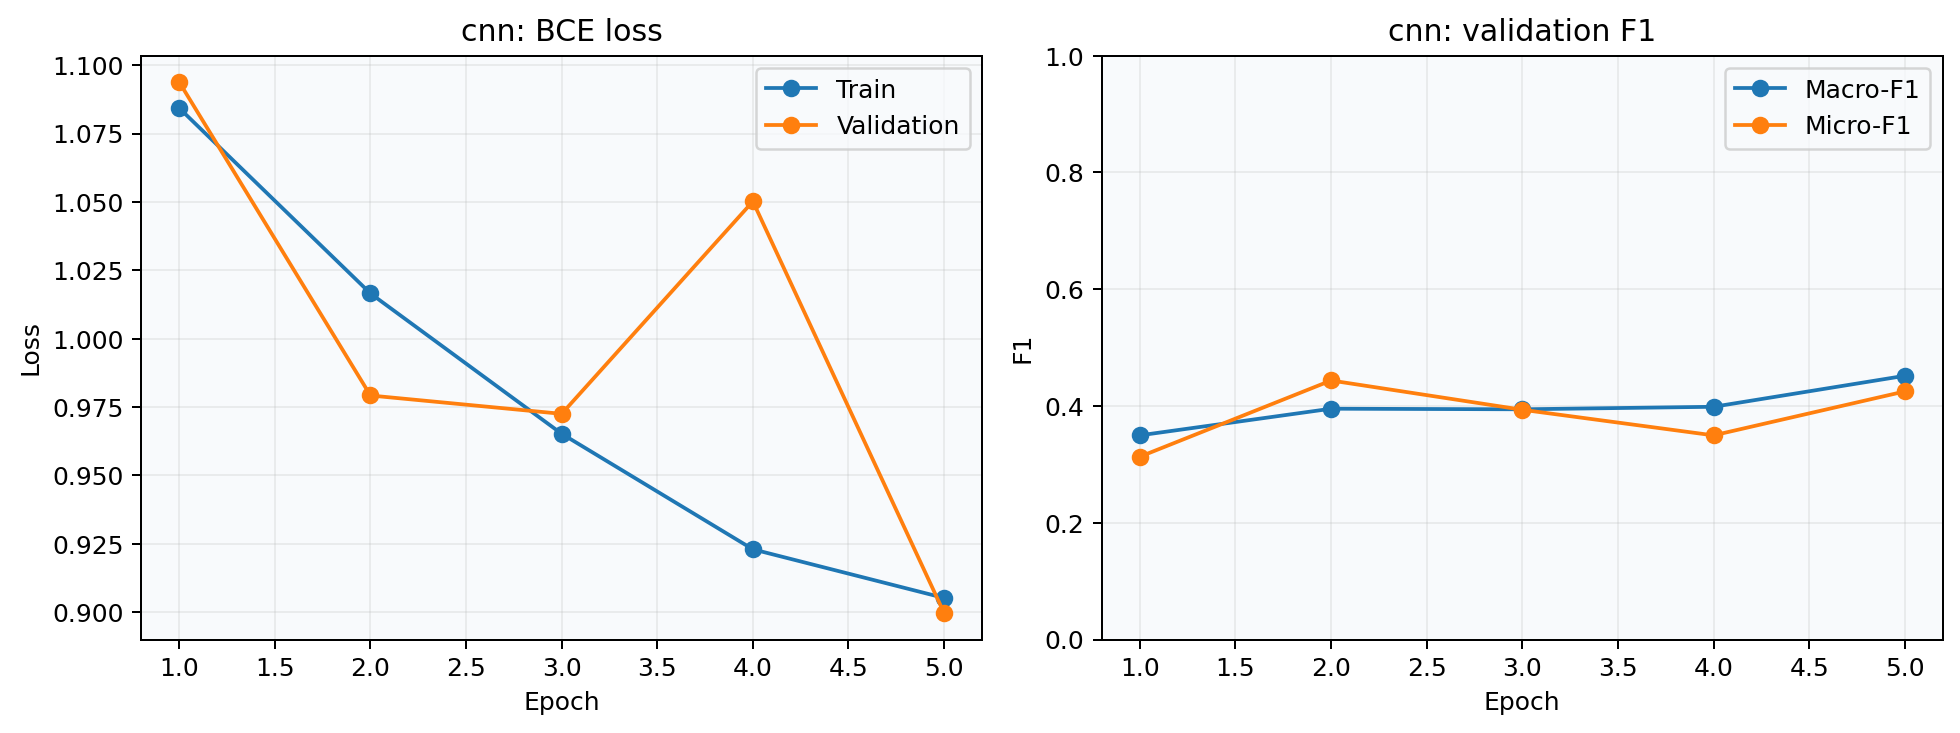
\includegraphics[width=0.31\textwidth]{../plots/cnn_training_curves.png}
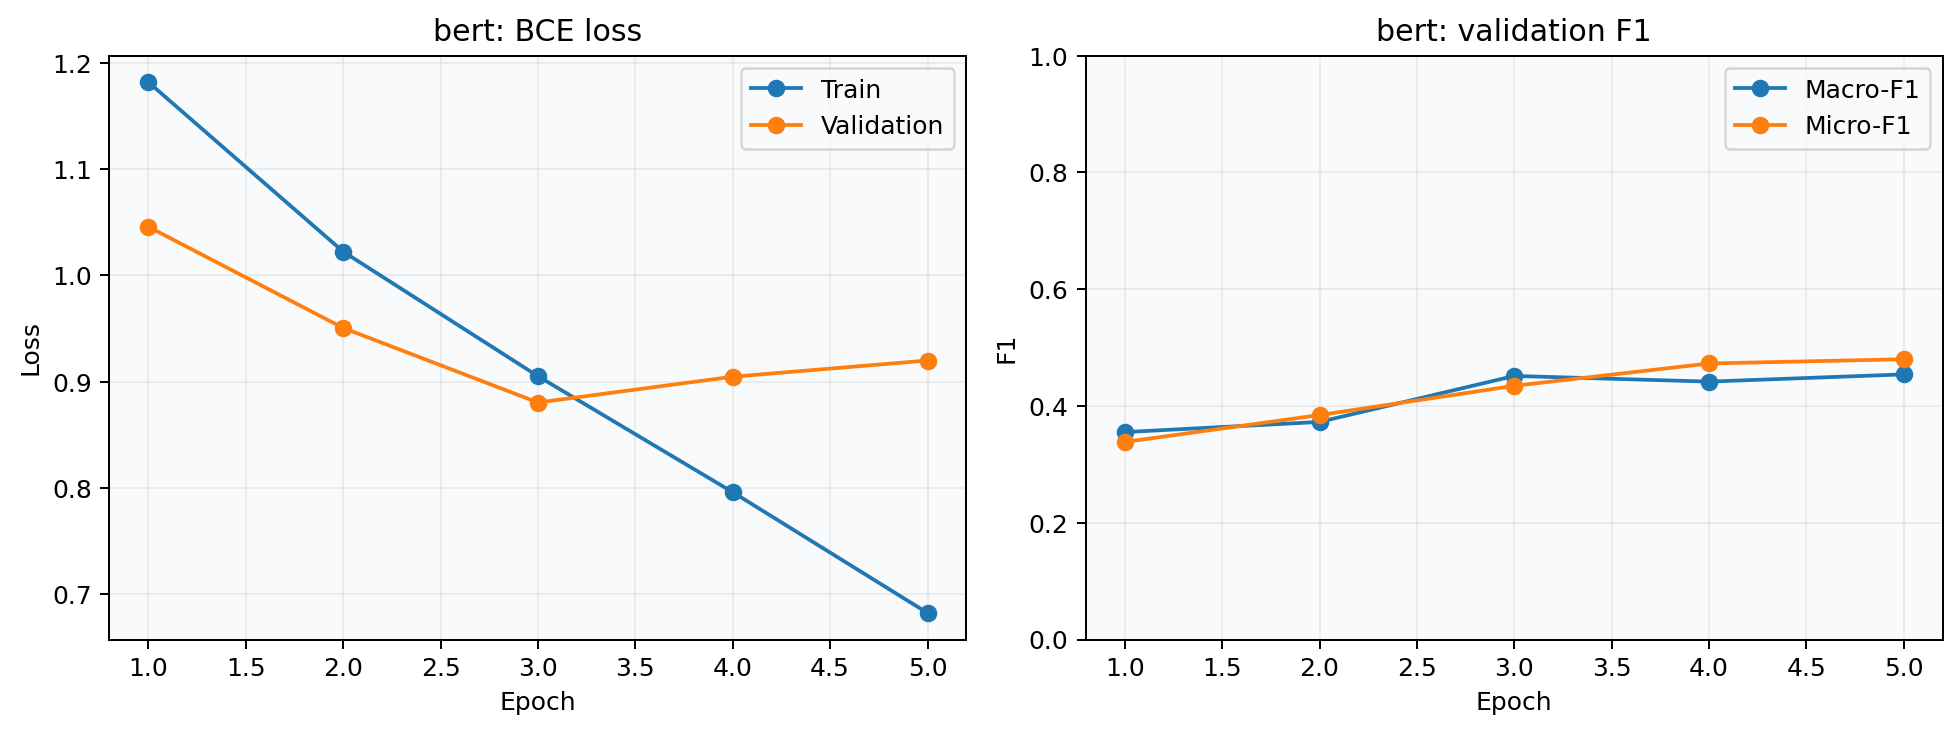
\includegraphics[width=0.31\textwidth]{../plots/bert_training_curves.png}
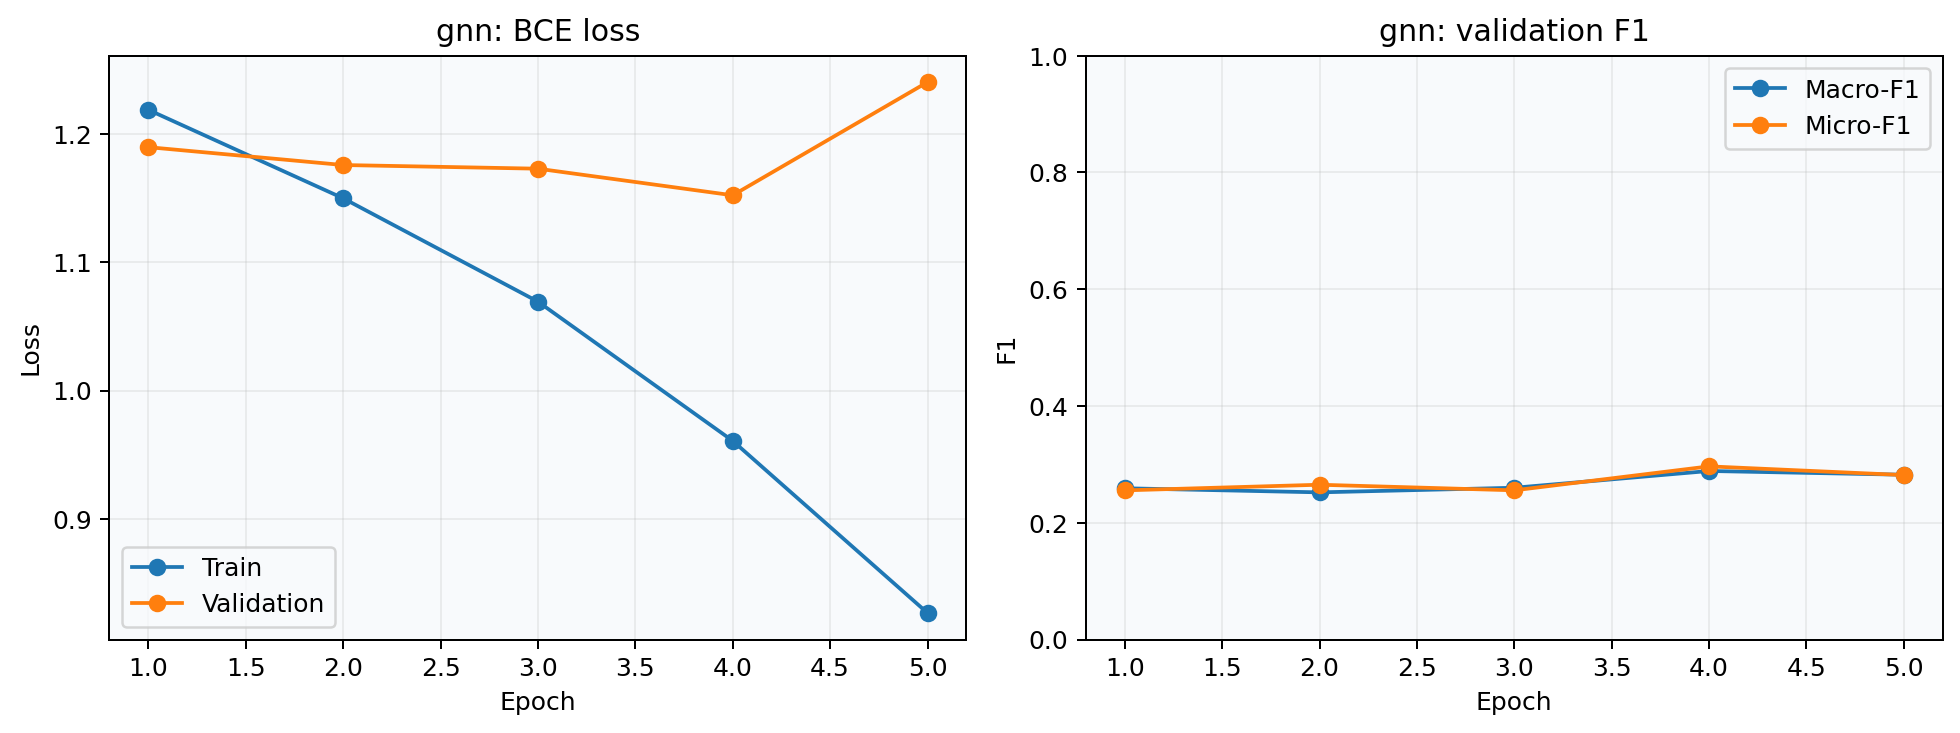
\includegraphics[width=0.31\textwidth]{../plots/gnn_training_curves.png}\\
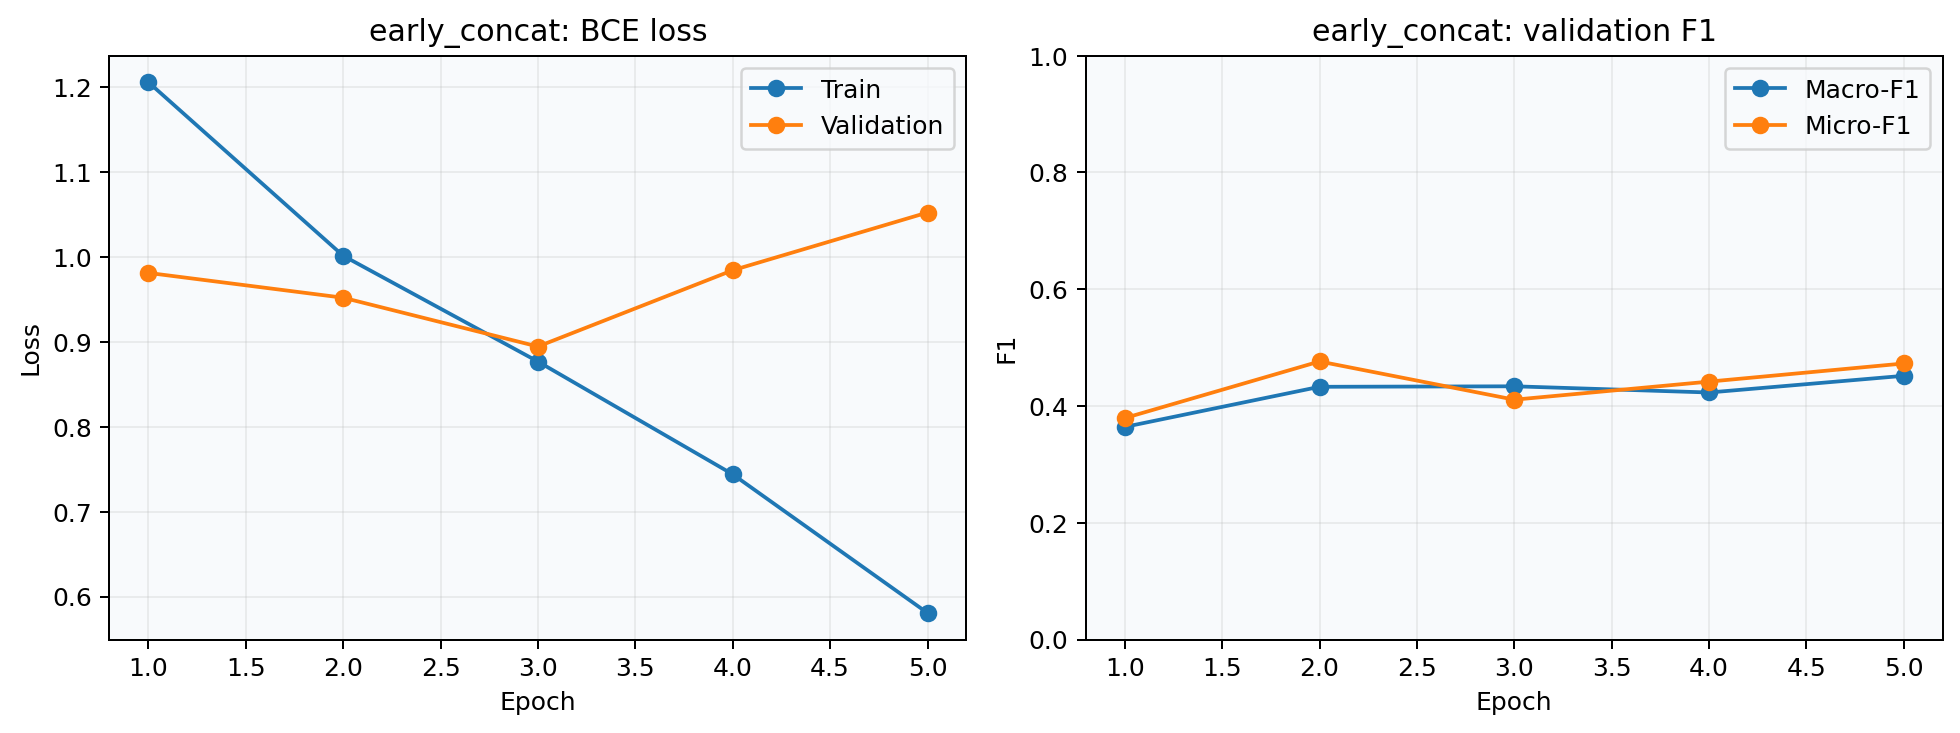
\includegraphics[width=0.31\textwidth]{../plots/early_concat_training_curves.png}
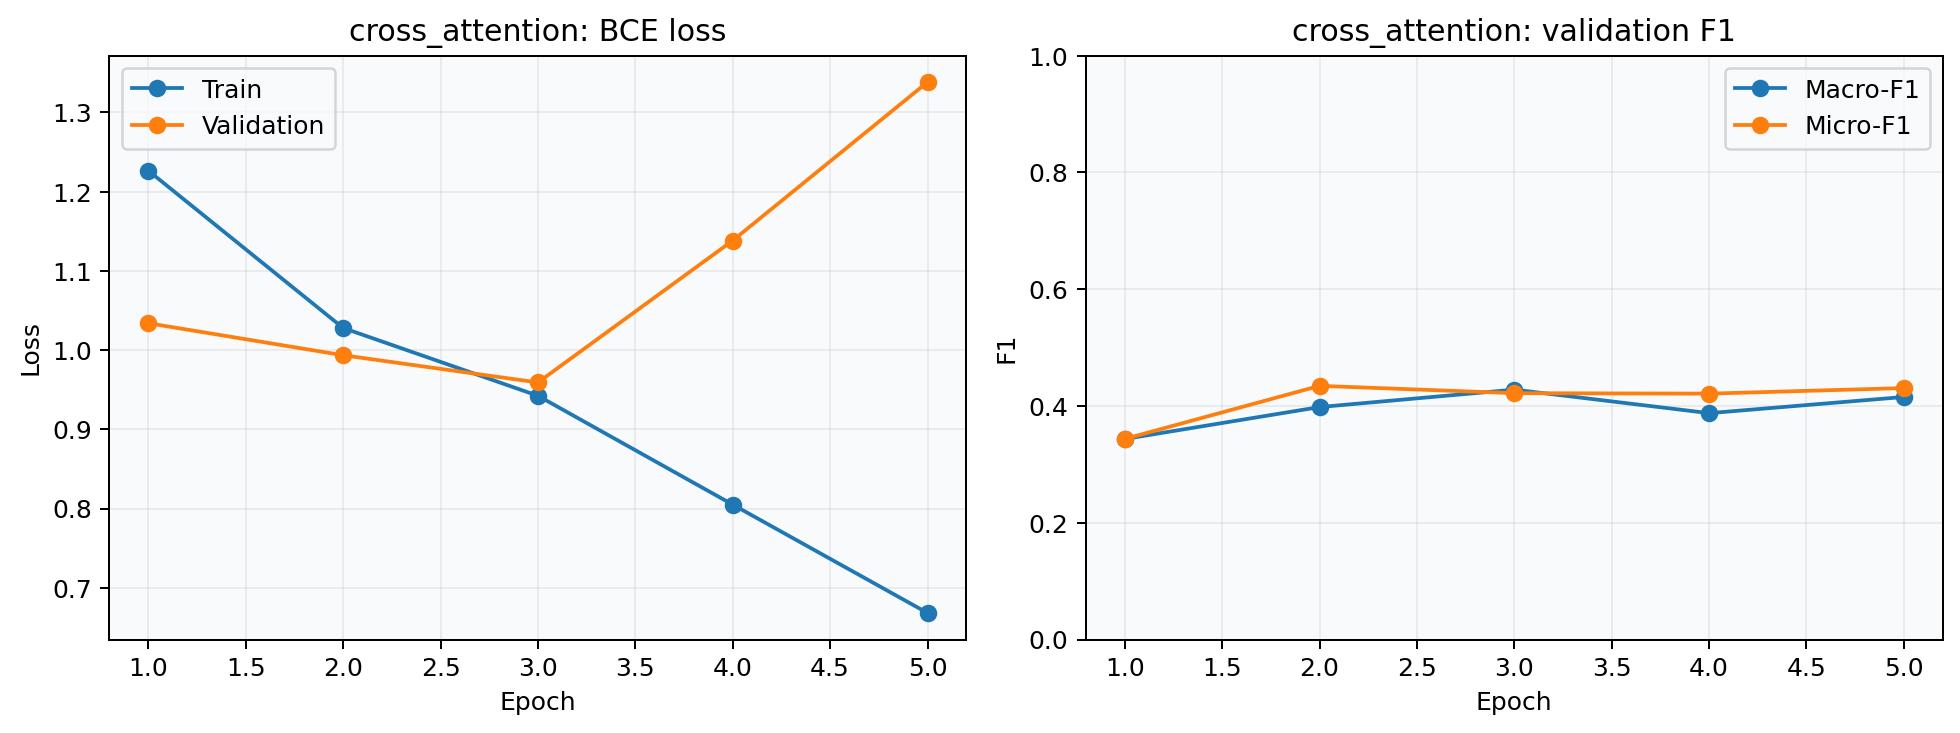
\includegraphics[width=0.31\textwidth]{../plots/cross_attention_training_curves.png}
\caption{Training and validation curves for the five learned models. The multimodal models begin to overfit within the five-epoch run, motivating validation-based checkpoint selection.}
\label{fig:curves}
\end{figure*}

\begin{figure}[t]
\centering
\IfFileExists{../plots/fusion_tsne.png}{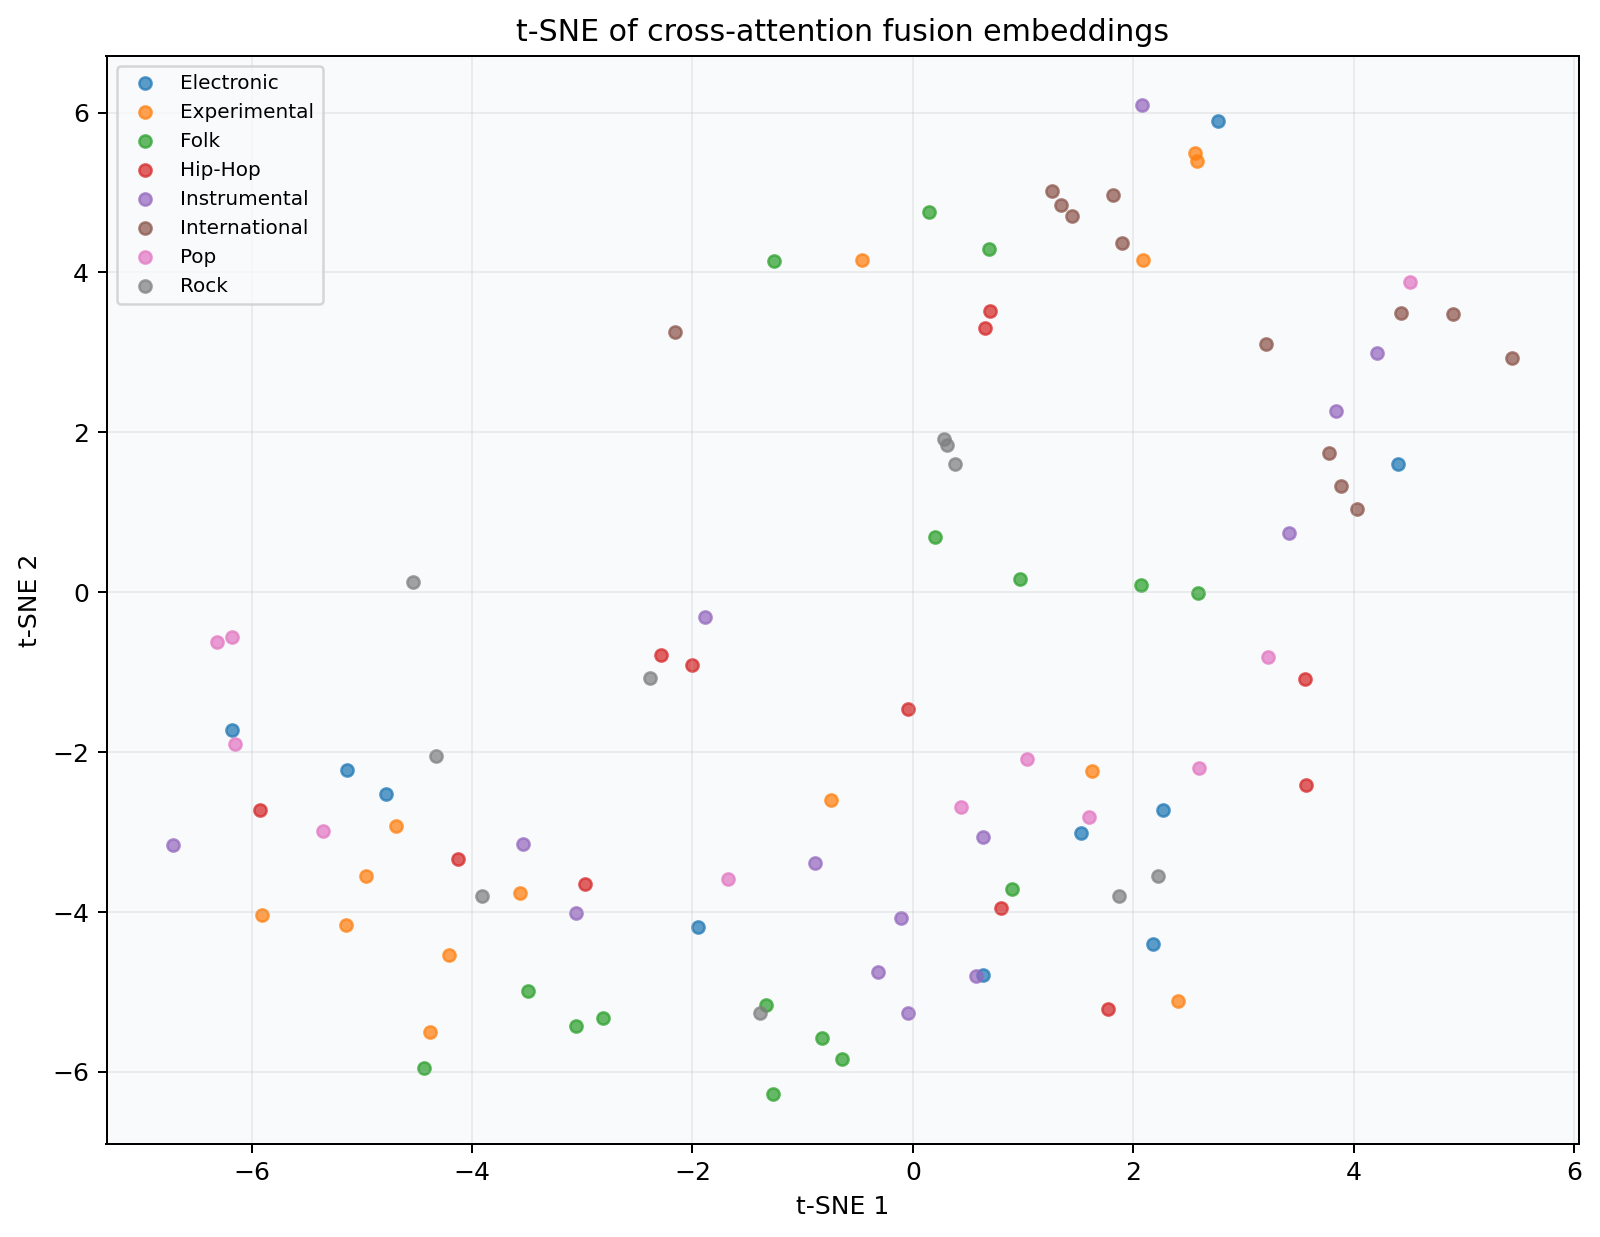
\includegraphics[width=\columnwidth]{../plots/fusion_tsne.png}}{\fbox{\parbox[c][1.8in][c]{0.9\columnwidth}{\centering t-SNE plot unavailable.}}}
\caption{t-SNE projection of cross-attention fusion embeddings, colored by the positive top-level genre.}
\label{fig:tsne}
\end{figure}

Figure~\ref{fig:tsne} shows limited but visible local grouping. Several International examples occupy the upper-right region, while groups of Folk examples appear near the lower and upper-center regions. Electronic, Experimental, Instrumental, Pop, and Rock remain substantially interleaved. This weak separation is consistent with the moderate cross-attention test score, although t-SNE can distort distances and is qualitative rather than a direct measure of classification quality.

\section{Qualitative Case Studies}
The three selected high-confidence cases are all correctly predicted as International with probabilities of 0.984, 0.983, and 0.983. Each graph contains six five-second nodes joined by temporal edges only; therefore these examples provide no evidence that non-adjacent similarity edges were decisive. In the first two cases the titles differ, but the album and artist are shared, and the model emphasizes ``at,'' ``the,'' ``live,'' and ``festival.'' The third case shows the same pattern, with 56.1\% of mean attention on ``at.'' Function words dominate over artist-specific tokens, so attention is not a convincing semantic explanation even though graph and text branches jointly yield the correct class. The repeated International examples also reveal selection bias in choosing only the most confident predictions. Attention weights show model emphasis, not causal importance.

\begin{figure*}[t]
\centering
\IfFileExists{../plots/case_study_1.png}{
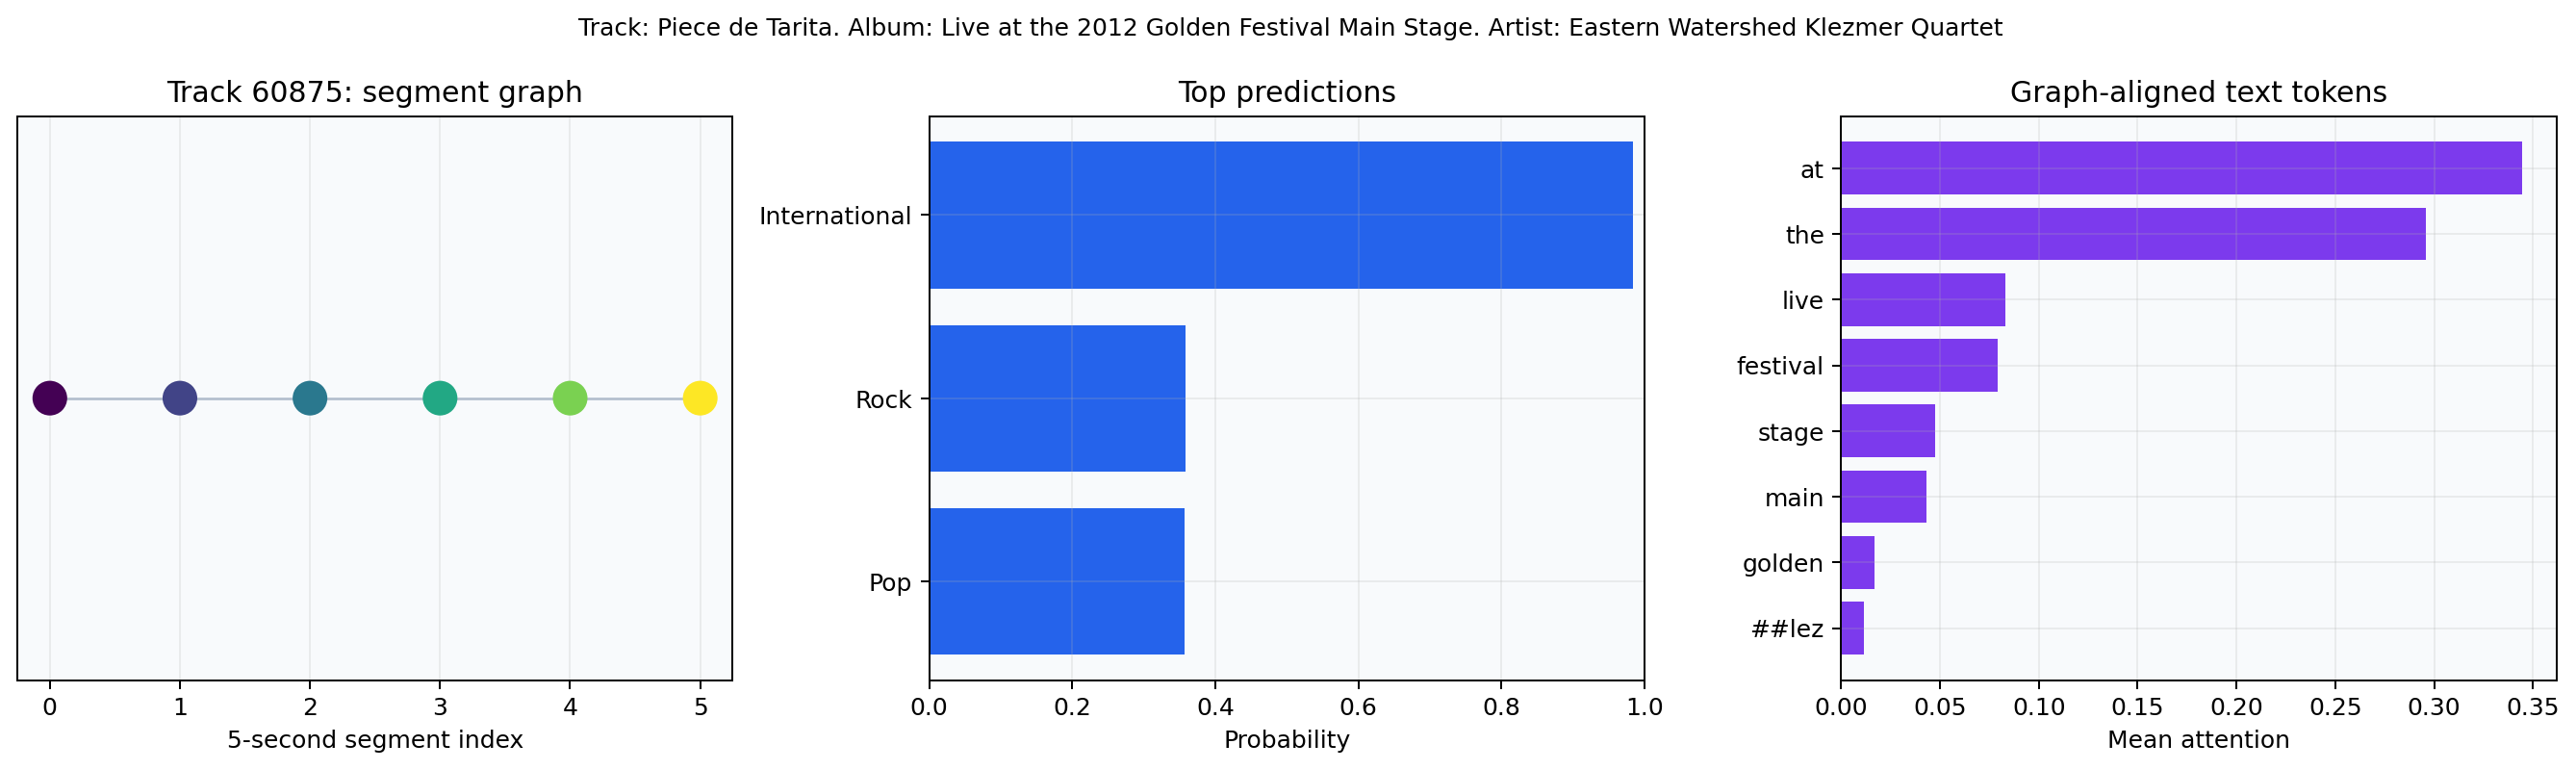
\includegraphics[width=0.32\textwidth]{../plots/case_study_1.png}
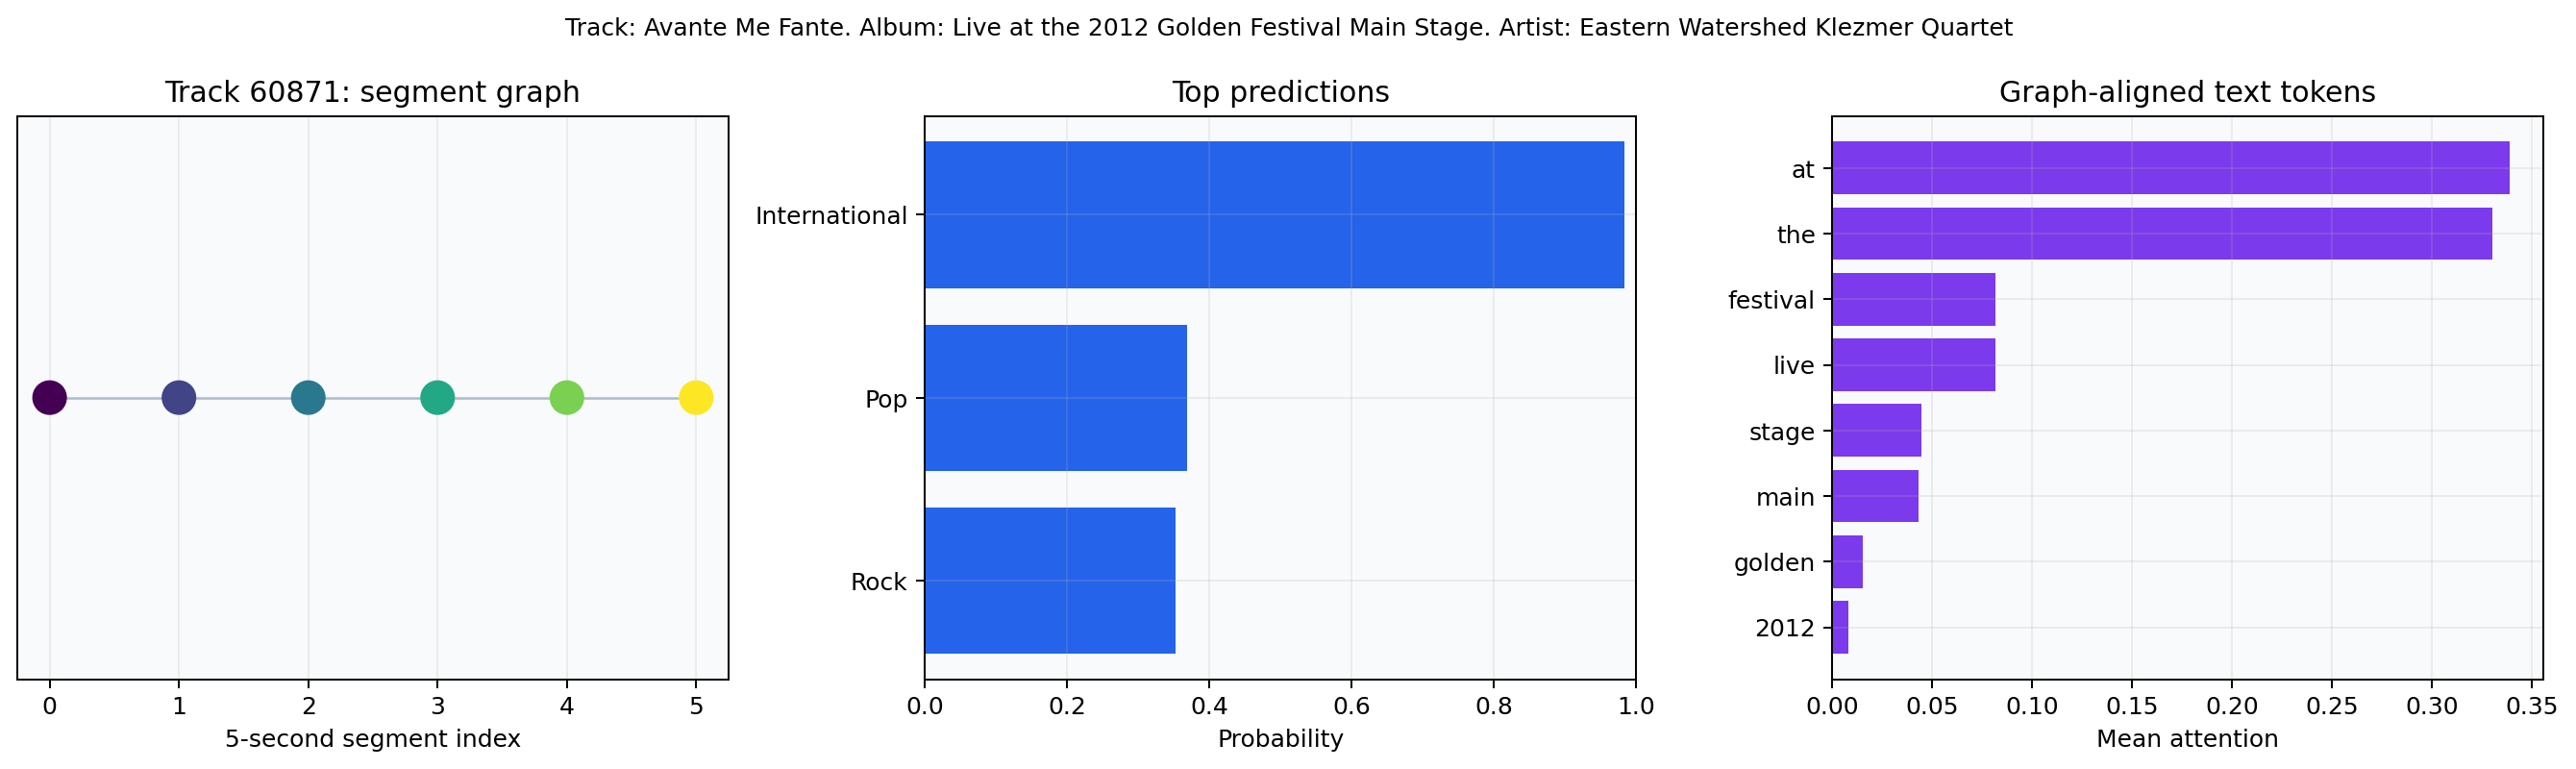
\includegraphics[width=0.32\textwidth]{../plots/case_study_2.png}
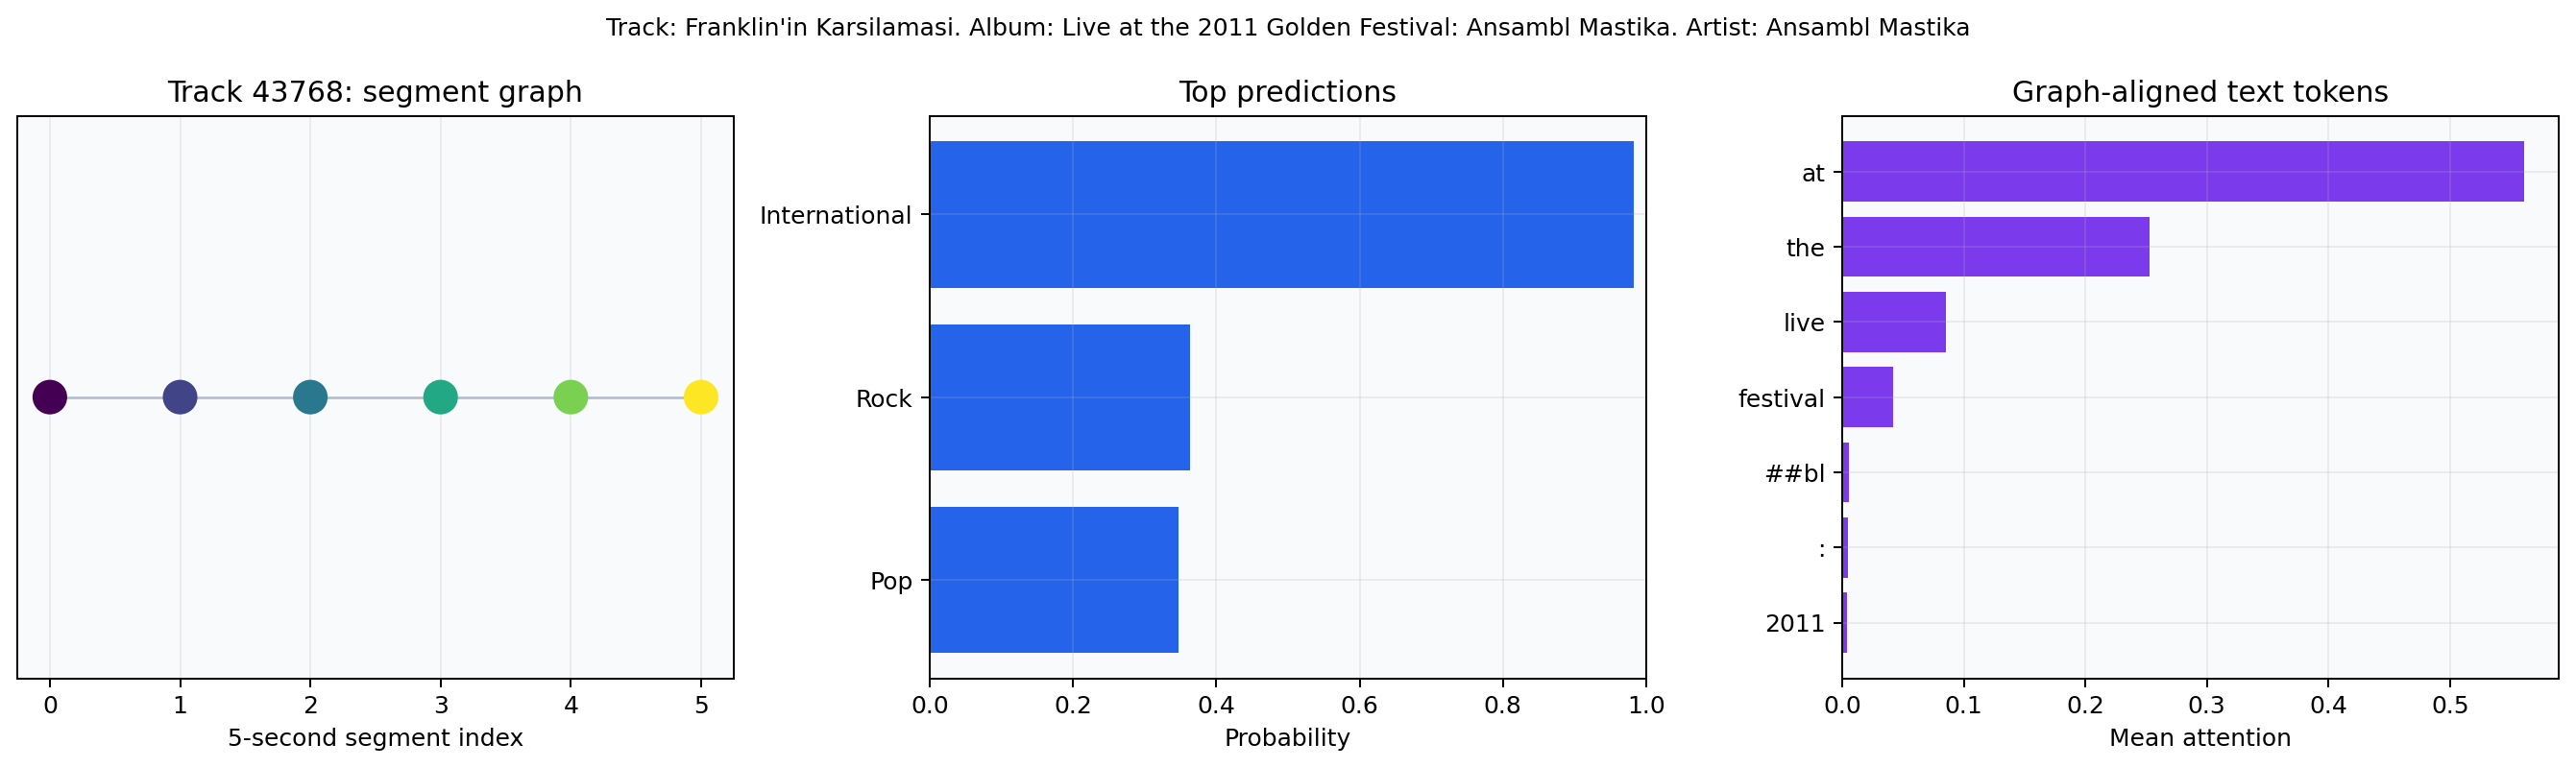
\includegraphics[width=0.32\textwidth]{../plots/case_study_3.png}
}{\fbox{\parbox[c][2.8in][c]{0.94\textwidth}{\centering Three case-study panels are generated after the cross-attention test run. Each panel contains the segment graph, top genre probabilities, and graph-aligned token attention.}}}
\caption{Three qualitative cross-attention cases. Each saved panel shows audio-segment connections, predicted context, and the text tokens receiving the strongest mean attention.}
\label{fig:cases}
\end{figure*}

\subsection{Error analysis protocol}
The stored probability arrays permit reproducible follow-up error inspection. Errors can be grouped into four hypotheses: acoustically related genres, sparse or uninformative text, artist correlation, and graph construction failure. The first can appear when instrumental and electronic textures overlap; the second when titles are generic; the third when artist identity is overused; and the fourth when uniform windows divide meaningful musical events. The per-label AUC-PR values support uneven difficulty: CNN AUC-PR ranges from 0.126 for Pop to 0.718 for Rock, while cross-attention ranges from 0.152 for Pop to 0.636 for International.

This grouping should remain diagnostic rather than speculative. Acoustic similarity is supported by graph edges and node embeddings; text weakness is supported by attention distributed over neutral tokens; artist correlation is checked with the split audit; and graph failure is checked by inspecting similarity edges. Examples that do not support a category should be reported as unresolved rather than forced into a narrative.

\section{Optional Contrastive Extension}
The repository includes a dual-encoder extension. A graph projection $\tilde{g}_i$ and text projection $\tilde{t}_i$ are L2-normalized and trained with a symmetric InfoNCE loss:
\begin{equation}
\mathcal{L}_{NCE}=\frac{1}{2N}\sum_i\left[-\log\frac{e^{\tilde{g}_i^\top\tilde{t}_i/\tau}}{\sum_j e^{\tilde{g}_i^\top\tilde{t}_j/\tau}}-\log\frac{e^{\tilde{t}_i^\top\tilde{g}_i/\tau}}{\sum_j e^{\tilde{t}_i^\top\tilde{g}_j/\tau}}\right].
\end{equation}
The evaluation reports text-to-graph and graph-to-text recall at 1, 5, and 10, plus ten query examples with the top three matches. When run on FMA metadata, this is only a structural-text retrieval proxy. It must not be presented as the assignment's full MusicCaps task, which requires genuine expert captions aligned to corresponding audio clips. The extension is disabled by default so that it cannot consume resources or be accidentally misreported.

\section{Discussion and Limitations}
The experiment isolates modality contributions through controlled ablation, but several limitations remain. First, title/album/artist strings are weaker than lyrics or expert captions. Fusion may therefore learn artist-to-genre correlations rather than broad musical semantics. Second, FMA-small provides top-level genre rather than explicit mood, valence, and arousal labels, so the result covers only part of ``multi-context'' understanding. Third, five-second uniform windows do not align perfectly with beats, bars, or chorus boundaries. Fourth, cosine threshold and top-$k$ graph construction are hand-selected hyperparameters. Fifth, an official track split does not necessarily eliminate artist-level overlap; the audit must be reported.

Future work should align MusicCaps descriptions with available clips, use DEAM for emotion regression, compare beat-synchronous nodes, and test GAT or weighted message passing. The optional symmetric InfoNCE module in the repository supports preliminary graph-text retrieval, but it should be reported as a proxy unless trained on genuine caption-audio pairs.

\subsection{Threats to validity}
Internal validity depends on identical examples reaching every model. A decode failure before manifest creation is acceptable because the row is removed globally; a failure inside only one model would invalidate the comparison. Hyperparameter parity is also imperfect because BERT uses a smaller learning rate and batch size than lightweight baselines, although these differences are necessary for stable fine-tuning. Repeated runs would be preferable to a single seed, but hosted-GPU limits may make three complete final repetitions expensive. If only one final run is feasible, this constraint should be stated.

External validity is limited by the FMA collection and top-level taxonomy. Results may not transfer to commercial catalogs, non-Western genres, long tracks, lyrics, or subjective mood judgments. Construct validity is limited because genre is used as a measurable proxy for broad musical context. t-SNE and attention plots are descriptive tools, not proof that learned features match human explanations. These constraints do not negate the controlled ablation but bound its interpretation.

\section{Conclusion}
We developed a complete supervised pipeline for musical context understanding using structured audio and contextual text. Segment graphs make temporal and repeated-section relations explicit, DistilBERT encodes leakage-safe metadata, and cross-attention permits graph-conditioned selection of textual evidence. The common evaluation pipeline, baselines, ablations, saved graph examples, and qualitative analyses make the comparison reproducible. On the reported test subset, the CNN was best with 0.382 Macro-F1 and 0.477 Macro AUC-PR. Fusion helped relative to either GNN-only or BERT-only---early concatenation reached 0.331 Macro-F1---but it did not outperform the stronger CNN acoustic baseline; cross-attention reached 0.298. This negative result is important evidence that sparse metadata and limited training data can outweigh the theoretical benefits of a more complex fusion mechanism.

\IfFileExists{IEEEtran.bst}{\bibliographystyle{IEEEtran}}{\bibliographystyle{plain}}
\bibliography{references}
\end{document}
